\documentclass[a4paper,10pt]{article}
\usepackage[utf8]{inputenc}
 
% Blank line between paragraphs instead of indenting the first line
\usepackage{parskip}
\setlength{\parskip}{\baselineskip}

% Squash a bit more text onto a page
\usepackage{geometry}
\geometry{verbose,tmargin=15mm,bmargin=15mm,lmargin=15mm,rmargin=15mm}

\usepackage{graphicx}
\usepackage{listings}
\usepackage{amsmath}
\usepackage{verbatim}
\usepackage{color}
\usepackage{wrapfig}

% Indent verbatim environments
\makeatletter \def\verbatim@processline{\hspace*{2em}\the\verbatim@line\par}\makeatother

\definecolor{mygreen}{rgb}{0,0.6,0}
\definecolor{mygray}{rgb}{0.5,0.5,0.5}
\definecolor{mymauve}{rgb}{0.58,0,0.82}

\lstset { 
  backgroundcolor=\color{white},   % choose the background color; you must add \usepackage{color} or \usepackage{xcolor}
  basicstyle=\footnotesize,        % the size of the fonts that are used for the code
  breakatwhitespace=false,         % sets if automatic breaks should only happen at whitespace
  breaklines=true,                 % sets automatic line breaking
  captionpos=b,                    % sets the caption-position to bottom
  commentstyle=\color{mygreen},    % comment style
  deletekeywords={...},            % if you want to delete keywords from the given language
  escapeinside={\%*}{*)},          % if you want to add LaTeX within your code
  extendedchars=true,              % lets you use non-ASCII characters; for 8-bits encodings only, does not work with UTF-8
  frame=single,                    % adds a frame around the code
  keepspaces=true,                 % keeps spaces in text, useful for keeping indentation of code (possibly needs columns=flexible)
  keywordstyle=\color{blue},       % keyword style
  language=C++,                    % the language of the code
  morekeywords={*,DEVICES,
  				CONNECTIONS,
  				MONITORS,
  				END}, 	           % if you want to add more keywords to the set
  numbers=left,                    % where to put the line-numbers; possible values are (none, left, right)
  numbersep=5pt,                   % how far the line-numbers are from the code
  numberstyle=\tiny\color{mygray}, % the style that is used for the line-numbers
  rulecolor=\color{black},         % if not set, the frame-color may be changed on line-breaks within not-black text (e.g. comments (green here))
  showspaces=false,                % show spaces everywhere adding particular underscores; it overrides 'showstringspaces'
  showstringspaces=false,          % underline spaces within strings only
  showtabs=false,                  % show tabs within strings adding particular underscores
  stepnumber=1,                    % the step between two line-numbers. If it's 1, each line will be numbered
  stringstyle=\color{mymauve},     % string literal style
  tabsize=2,                       % sets default tabsize to 2 spaces
  title=\lstname                   % show the filename of files included with \lstinputlisting; also try caption instead of title
}

\begin{document}

\begin{center}
\LARGE \textbf{IIA GF2 Software: 2nd Interim Report}

\small Tim Hillel (th389) - Team 8
\end{center}

\section{User Guide}
\begin{description}
\item[1. Open logic simulator] \hspace{0.1em}
\begin{description}
 \item[Using terminal]\hfill \\
Open a terminal and setting the directory to the \texttt{./logsim/src} folder. Start the application by entering \texttt{./logsim}. To open a known definition file, follow this by the directory of the definiton file, and skip instruction 2.
 \item[Using file browser]\hfill \\ 
Browse to \texttt{./logsim/src} and double click on the \texttt{logsim} executable file.
\end{description}
\item[2. Open definition file]\hfill \\ 
Click \texttt{File} menu and select \texttt{Open} to open the file selection dialogue. Only definition files with the extension \texttt{.gf2} will be displayed. The default directory is \texttt{./examples}. Browse to the required definition file and double click to open it.
\item[3. Errors]\hfill \\
If the definition file contains errors, the message \texttt{Failed to load file} will display in the display panel and any errors in the definition file will be written to the message window. If there are no errors the message \texttt{No simulation results. Use the run button.} will display, and the simulator is ready to run.
\item[4. Run simulation]\hfill \\
Enter a number of clock cycles required in the \texttt{Simulation} box, either using the up and down arrows or entering the number as text. The default value is 42. Click run once the required value has been entered.
\item [5. Output]\hfill \\
The monitored signals will be displayed in the left display panel. The simulation can be continued by the specified number of clock cycles by pressing the continue button. This can be repeated multiple times. Scrollbars will appear once there is too much data to display in the display panel; these can be used to scroll across the display.
\item[6. Change switch states]\hfill \\
Click the check box next to a switch in the \texttt{Switches} box to change its state (ticked box will be high, unticked low). Run or continue the simulation to see the effect on the circuit.
\item[7. Add monitors]\hfill \\
Click the \texttt{Add monitors} button to open the dialogue box. Select the desired output(s) to monitor and then click \texttt{OK} to add these outputs to the display panel. Mulitple outputs can be selected by holding the \texttt{ctrl} button.
\item[8. Remove monitors]
To remove monitors, clock the \texttt{Remove monitors} button to open the dialogue box. Select the desired monitor(s) to remove and then click \texttt{OK}. Mulitple outputs can be selected by holding the \texttt{ctrl} button. The selected monitors will be removed from the display panel.
\item[9. Edit devices]\hfill \\
Click the \texttt{Edit devices} button to open the dialogue box. Select the required device to edit in the left hand panel, and use the options within the dialogue box to change the device name, type and number of inputs (if applicable).
\end{description}

Note that changes made in steps 6-9 will only make changes within the simulation and will not change the definition files.

\pagebreak

\section{Test Definition Files}

\subsection{XOR Gate}
\subsubsection{Definition File}
\lstinputlisting[caption=xor.gf2]{../../examples/xor.gf2}
\subsubsection{Circuit Diagram}
\begin{figure}[h]
 \centering
 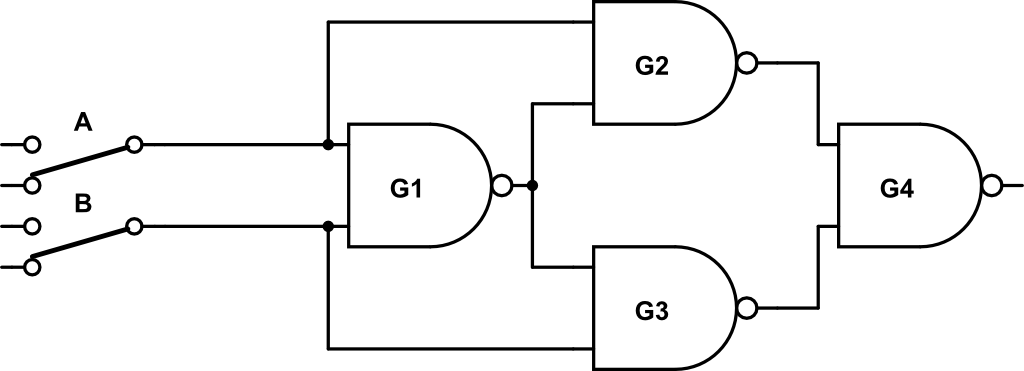
\includegraphics[width=8cm]{../../examples/xor.png}
 \caption{Circuit diagram of an XOR gate implemented using NAND gates}
 \label{fig:example-xor}
\end{figure}

\subsection{4-bit Adder}
\subsubsection{Definition File}
\lstinputlisting[caption=4bitadder.gf2]{../../examples/4bitadder.gf2}
\subsubsection{Circuit Diagram}
\begin{figure}[h]
 \centering
 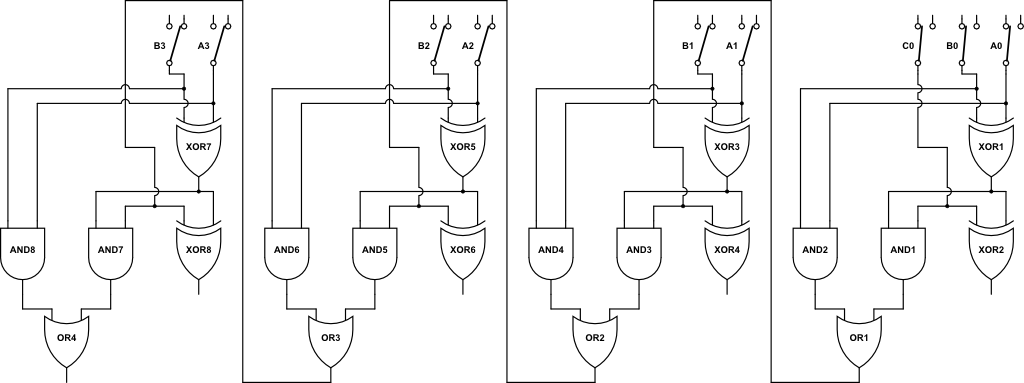
\includegraphics[width=16cm]{../../examples/4-bit-adder.png}
 \caption{Circuit diagram of a 4-bit adder}
 \label{fig:example-adder}
\end{figure}

\subsection{Serial In Parallel Out Shift Register}
\subsubsection{Definition File}
\lstinputlisting[caption=sipo.gf2]{../../examples/sipo.gf2}
\subsubsection{Circuit Diagram}

\begin{figure}[h]
 \centering
 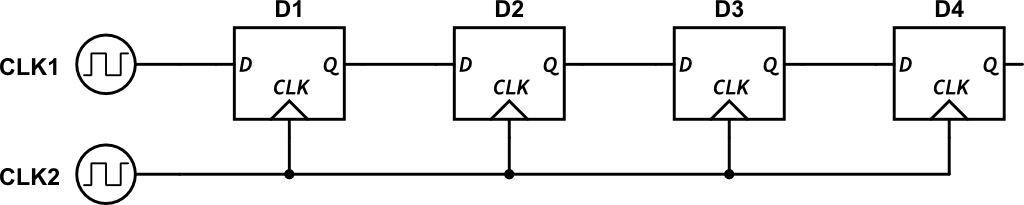
\includegraphics[width=12cm]{../../examples/sipo.png}
 \caption{Circuit diagram of a serial in parallel out shift register}
 \label{fig:example-sipo}
\end{figure}

\textbf{NB} The software used to draw the circuit diagram does not support the same style of D flip-flop used in the definition file, and Fig. \ref{fig:example-sipo} was the closest achievable.

\subsection{Gated D Latch}
\subsubsection{Definition File}
\lstinputlisting[caption=sipo.gf2]{../../examples/gateddlatch.gf2}
\subsubsection{Circuit Diagram}
\begin{figure}[h]
 \centering
 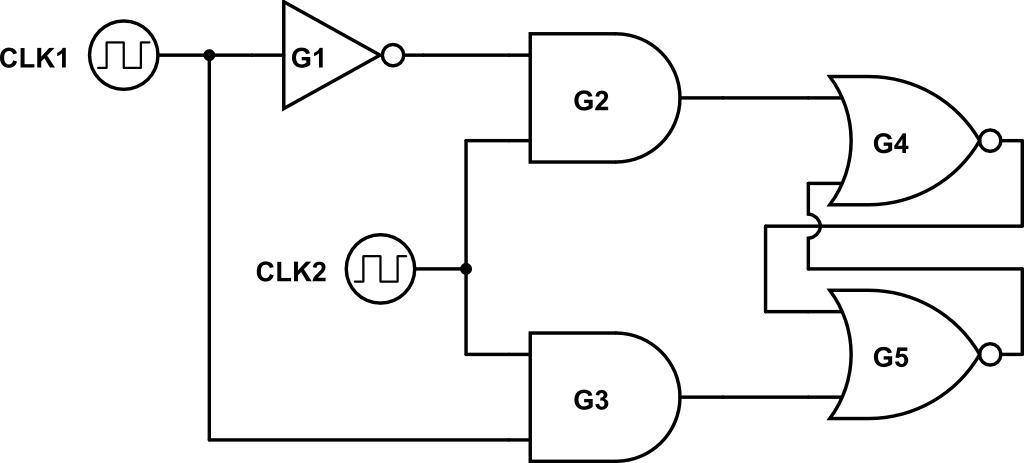
\includegraphics[width=12cm]{../../examples/gated-d-latch.png}
 \caption{Circuit diagram of a Gated D Latch}
 \label{fig:example-dlatch}
\end{figure}

\textbf{NB} The software used to draw the circuit diagram does not support the NAND gates with one input. Therefore the NAND gate G1 was substituted for a NOT gate as can be seen in Fig. \ref{fig:example-dlatch}.

\pagebreak

\section{Code Listings}
\subsection{Parser Class}
\subsubsection{parser.h}
\lstinputlisting[caption=parser.h]{../../src/parser.h}
\subsubsection{parser.cc}
\lstinputlisting[caption=parser.cc]{../../src/parser.cc}

I was mainly responsible for \texttt{parser.cc}, with input from Jamie Magee on the \texttt{connectionList} and \texttt{monitorList} functions. (Final ratio was around 80\% my work, 20\% his work.) 

\subsection{Error Class}
\subsubsection{error.h}
\lstinputlisting[caption=error.h]{../../src/error.h}
\subsubsection{error.cc}
\lstinputlisting[caption=error.cc]{../../src/error.cc}


\end{document}
